\section{Forward Model Impact}
%=============================

\subsection{Clouds}
%------------------
The brightness temperature residuals that result from using different schemes for interpolation of the cloud optical properties for the test cloud profiles for NOAA-18 HIRS/4, NOAA-18 AMSU-A, and Band 1 of MetOp-A IASI are shown in figures \ref{fig:hirs4_n18.Differences.FWD.Cloud}, \ref{fig:amsua_n18.Differences.FWD.Cloud}, and \ref{fig:iasiB1_metop-a.Differences.FWD.Cloud} respectively.

Comparison of the clear-cloudy residuals to the interpolation residuals indicates that the latter is a small fraction of the former, but the magnitudes of the interpolation residuals can be relatively large, e.g. HIRS/4 and IASI hail and rain cloud cases, and AMSU-A ch.15 for most cloud cases. In addition, primarily for the infrared instruments, the differences between interpolation schemes alone can be relatively large which suggests that the residuals are overly influenced by anomalous interpolation due to low LUT data density. However, the interpretation of the interpolation residuals is somewhat complicated by the fact that the cloud optical properties used in the current CRTM version do not cover all the ranges of input data (e.g. effective radii, temperatures). This is discussed further in section  \ref{sec:Insufficient.LUT.range.Cloud}.
 
\begin{figure}[htp]
  \centering
  \textsf{\textbf{NOAA-18 HIRS/4}}\vspace{1.5ex}
  \includegraphics[bb=70 130 540 646,clip,scale=1.0]{graphics/Cloud/FWD/hirs4_n18.Differences.eps}
  \caption{Cloudy brightness temperature residuals for NOAA-18 HIRS/4. \textbf{(Left column)} Clear - Cloudy brightness temperature residuals. \textbf{(Centre column)} Cloudy calculation residuals due to difference in interpolated cloud optical properties from linear and cubic interpolation schemes. \textbf{(Right column)} Cloudy calculation residuals due to difference in interpolated cloud optical properties from linear and averaged quadratic interpolation schemes.}
  \label{fig:hirs4_n18.Differences.FWD.Cloud}
\end{figure}

\begin{figure}[htp]
  \centering
  \textsf{\textbf{NOAA-18 AMSU-A}}\vspace{1.5ex}
  \includegraphics[bb=70 130 540 646,clip,scale=1.0]{graphics/Cloud/FWD/amsua_n18.Differences.eps}
  \caption{Cloudy brightness temperature residuals for NOAA-18 AMSU-A. \textbf{(Left column)} Clear - Cloudy brightness temperature residuals. \textbf{(Centre column)} Cloudy calculation residuals due to difference in interpolated cloud optical properties from linear and cubic interpolation schemes. \textbf{(Right column)} Cloudy calculation residuals due to difference in interpolated cloud optical properties from linear and averaged quadratic interpolation schemes.}
  \label{fig:amsua_n18.Differences.FWD.Cloud}
\end{figure}

\begin{figure}[htp]
  \centering
  \textsf{\textbf{MetOp-A IASI (Band 1)}}\vspace{1.5ex}
  \includegraphics[bb=70 130 540 646,clip,scale=1.0]{graphics/Cloud/FWD/iasiB1_metop-a.Differences.eps}
  \caption{Cloudy brightness temperature residuals for MetOp-A IASI Band 1. \textbf{(Left column)} Clear - Cloudy brightness temperature residuals. \textbf{(Centre column)} Cloudy calculation residuals due to difference in interpolated cloud optical properties from linear and cubic  interpolation schemes. \textbf{(Right column)} Cloudy calculation residuals due to difference in interpolated cloud optical properties from linear and averaged quadratic interpolation schemes.}
  \label{fig:iasiB1_metop-a.Differences.FWD.Cloud}
\end{figure}

\subsection{Aerosols}
%--------------------
The brightness temperature residuals that result from different schemes for interpolation of the aerosol optical properties for the test aerosol profiles for NOAA-18 HIRS/4 and Band 1 of MetOp-A IASI are shown in figures \ref{fig:hirs4_n18.Differences.FWD.Aerosol} and \ref{fig:iasiB1_metop-a.Differences.FWD.Aerosol} respectively.

Compared to the cloudy interpolation residuals, the magnitudes of the same for aerosol optical properties is negligible. This could be a result of using a too-low aerosol burden in the test profiles. Alternatively, it could also indicate that the aerosol optical properties are either smoother in general with respect to the independent variables, or that they are simply more effectively represented in the LUT. The similarity between the residuals regardless of the interpolation scheme suggests the latter.

\begin{figure}[htp]
  \centering
  \textsf{\textbf{NOAA-18 HIRS/4}}\vspace{1.5ex}
  \includegraphics[bb=70 130 540 646,clip,scale=1.0]{graphics/Aerosol/FWD/hirs4_n18.Differences.eps}
  \caption{Aerosol brightness temperature residuals for NOAA-18 HIRS/4. \textbf{(Left column)} Clear - Aerosol brightness temperature residuals. \textbf{(Centre column)} Aerosol calculation residuals due to difference in interpolated aerosol optical properties from linear and cubic interpolation schemes. \textbf{(Right column)} Aerosol calculation residuals due to difference in interpolated aerosol optical properties from linear and averaged quadratic interpolation schemes.}
  \label{fig:hirs4_n18.Differences.FWD.Aerosol}
\end{figure}

\begin{figure}[htp]
  \centering
  \textsf{\textbf{MetOp-A IASI (Band 1)}}\vspace{1.5ex}
  \includegraphics[bb=70 130 540 646,clip,scale=1.0]{graphics/Aerosol/FWD/iasiB1_metop-a.Differences.eps}
  \caption{Aerosol brightness temperature residuals for MetOp-A IASI Band 1. \textbf{(Left column)} Clear - Aerosol brightness temperature residuals. \textbf{(Centre column)} Aerosol calculation residuals due to difference in interpolated aerosol optical properties from linear and cubic  interpolation schemes. \textbf{(Right column)} Aerosol calculation residuals due to difference in interpolated aerosol optical properties from linear and averaged quadratic interpolation schemes.}
  \label{fig:iasiB1_metop-a.Differences.FWD.Aerosol}
\end{figure}

